\title{%
  Hello World!
}
\author{Daniel Bosk}
\institute{%
  KTH EECS
}

\mode<article>{\maketitle}
\mode<presentation>{%
  \begin{frame}
    \maketitle
  \end{frame}
}

\mode*

\begin{abstract}
  % What's the problem?
% Why is it a problem? Research gap left by other approaches?
% Why is it important? Why care?
% What's the approach? How to solve the problem?
% What's the findings? How was it evaluated, what are the results, limitations, 
% what remains to be done?

% XXX Summary
\emph{Summary:}
\dots

% XXX Motivation and intended learning outcomes
\emph{Intended learning outcomes:}
\dots

% XXX Prerequisites
\emph{Prerequisites:}
\dots

% XXX Reading material
\emph{Reading:}
\dots

\end{abstract}


\section{Programmering}

\subsection{Vad är programmering?}

\begin{frame}
  \begin{block}{Dator}
    \begin{itemize}
      \item Processor
      \item Minne
      \item Annan hårdvara
    \end{itemize}
  \end{block}
\end{frame}

\begin{frame}
  \begin{block}{Processorn}
    \begin{itemize}
      \item Exekverar maskinkod --- program
    \end{itemize}
  \end{block}

  \pause

  \begin{example}
    \begin{itemize}
      \item<1-2> 00012000050000020500
      \item<3-> 0001 2000 0500
      \item<3-> 0002 0500
    \end{itemize}
  \end{example}
\end{frame}

\begin{frame}
  \begin{block}{Svar}
    \begin{itemize}
      \item Programmering är att skriva program.
    \end{itemize}
  \end{block}
\end{frame}


\subsection{Programmeringsspråk}

\begin{frame}
  \begin{block}{Programmeringsspråk}
    \begin{itemize}
      \item Ett språk för människor att skriva datorprogram.
    \end{itemize}
  \end{block}
\end{frame}

\begin{frame}[fragile]
  \begin{example}[Python]
    \begin{minted}{python}
print("Hello, World!")
    \end{minted}
  \end{example}

  \pause

  \begin{example}[C++]
    \begin{minted}{c++}
#include <iostream>
using namespace std;

int main(void) {
    std::cout << "Hello, World!" << std::endl;
    return 0;
}
    \end{minted}
  \end{example}
\end{frame}

\begin{frame}
  \begin{remark}
    \begin{itemize}
      \item C++ måste översättas till maskinkod!
      \item Python läses av ett program (maskinkod), och det programmet 
        exekverar koden.
    \end{itemize}
  \end{remark}
\end{frame}

\begin{frame}[fragile]
  \begin{example}[Terminalen]
    \begin{minted}{bash}
echo "Hello World!"
    \end{minted}
  \end{example}

  \pause

  \begin{remark}
    \begin{itemize}
      \item Bash läser varje rad och exekverar olika program.
      \item Dessa program är redan konverterade till maskinkod.
    \end{itemize}
  \end{remark}
\end{frame}


\section{Köra Python}

\subsection{Terminalen}

\begin{frame}
  \begin{figure}
    \centering
    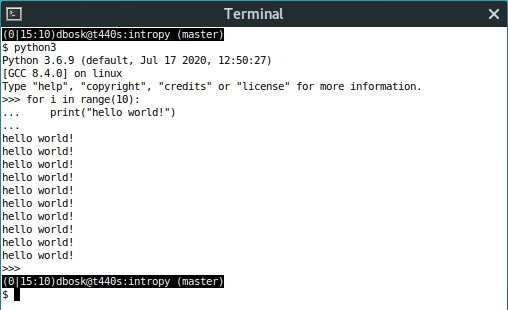
\includegraphics[height=0.8\textheight]{figs/python-terminal.png}
    \caption{Ett kodexempel i Python som skriver ut \enquote{hello world!} i 
    terminalen.}
  \end{figure}
\end{frame}


\subsection{Andra gränssnitt}

\begin{frame}
  \begin{figure}
    \centering
    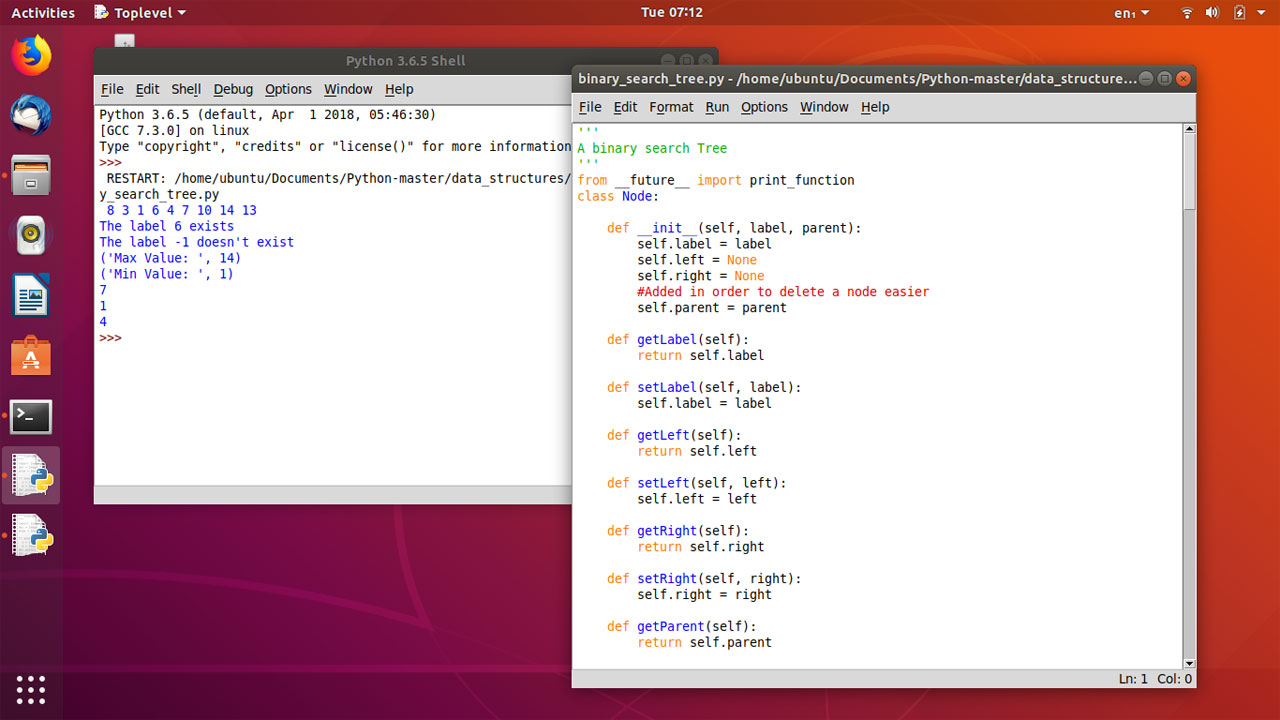
\includegraphics[height=0.8\textheight]{figs/idle.jpg}
    \caption{Kod och körning av pythonkod i Idle.}
  \end{figure}
\end{frame}

\begin{frame}
  \begin{figure}
    \centering
    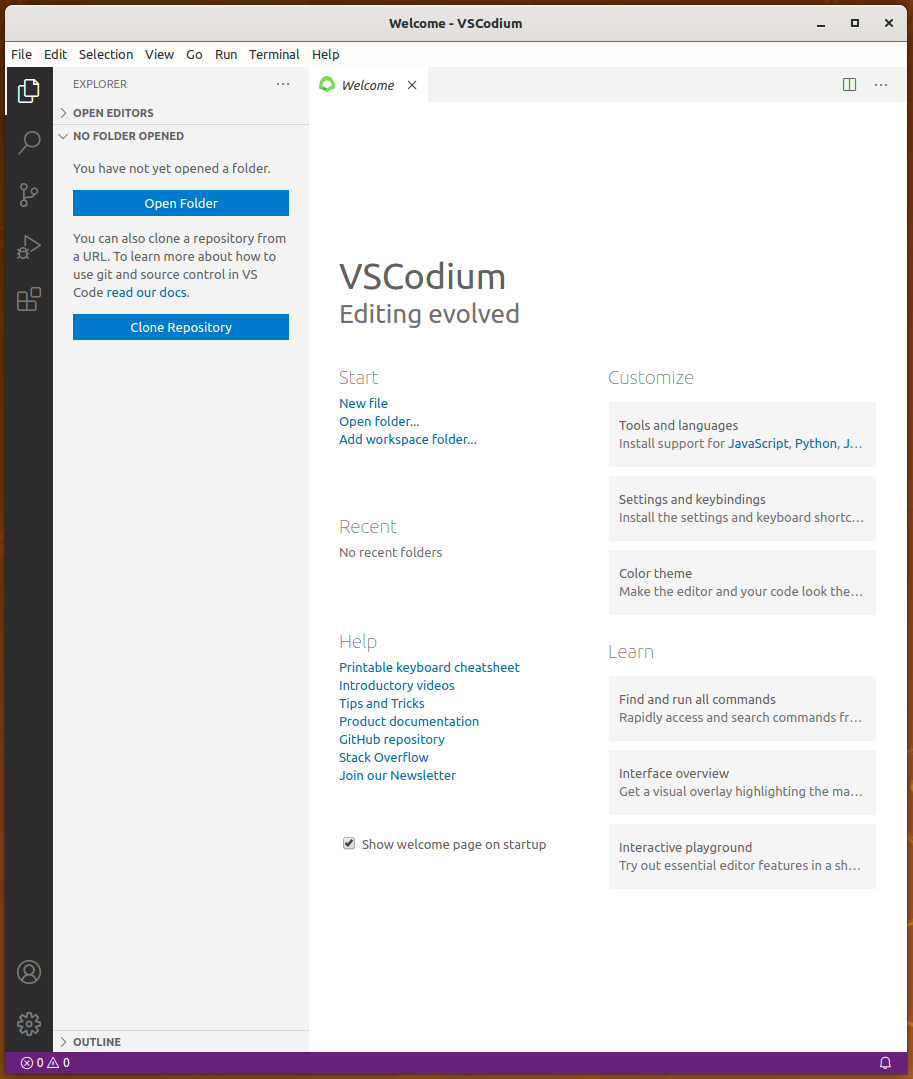
\includegraphics[height=0.8\textheight]{figs/codium.png}
    \caption{Gränssnittet till VSCodium (öppen källkodsvariant av Visual Studio 
    Code).}
  \end{figure}
\end{frame}

\begin{frame}
  \begin{figure}
    \centering
    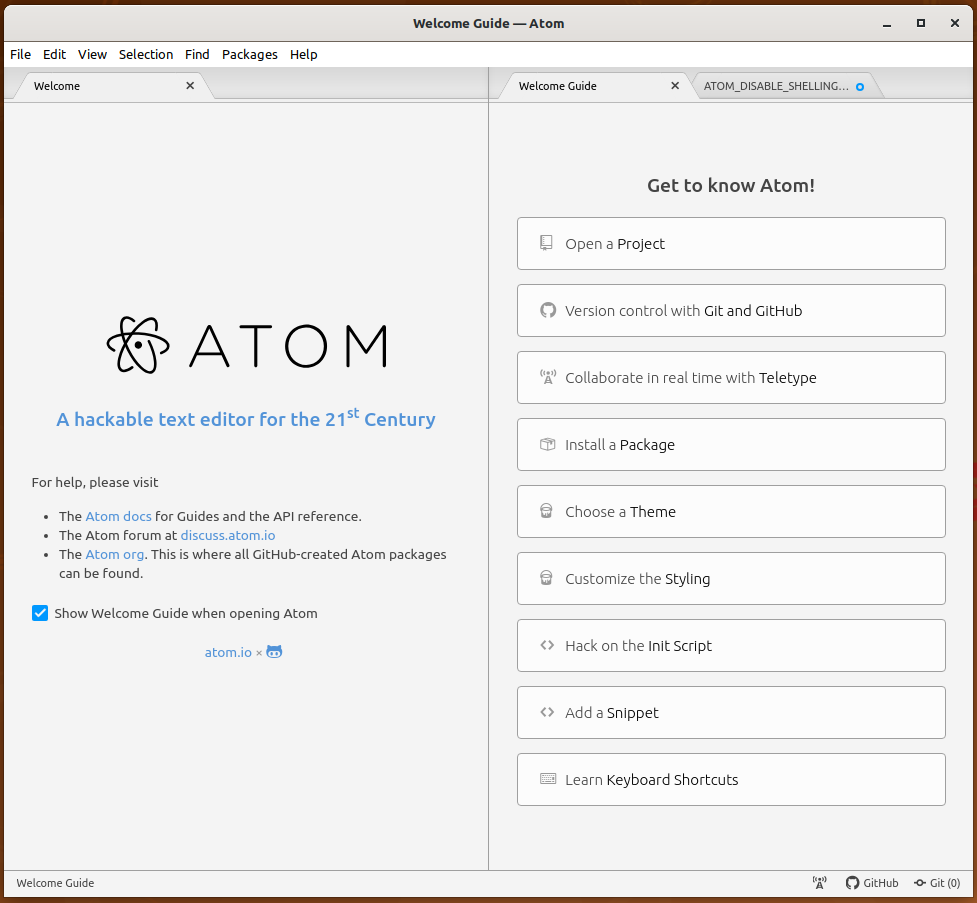
\includegraphics[height=0.8\textheight]{figs/atom.png}
    \caption{Gränssnittet för Atom.}
  \end{figure}
\end{frame}

\begin{frame}
  \begin{figure}
    \centering
    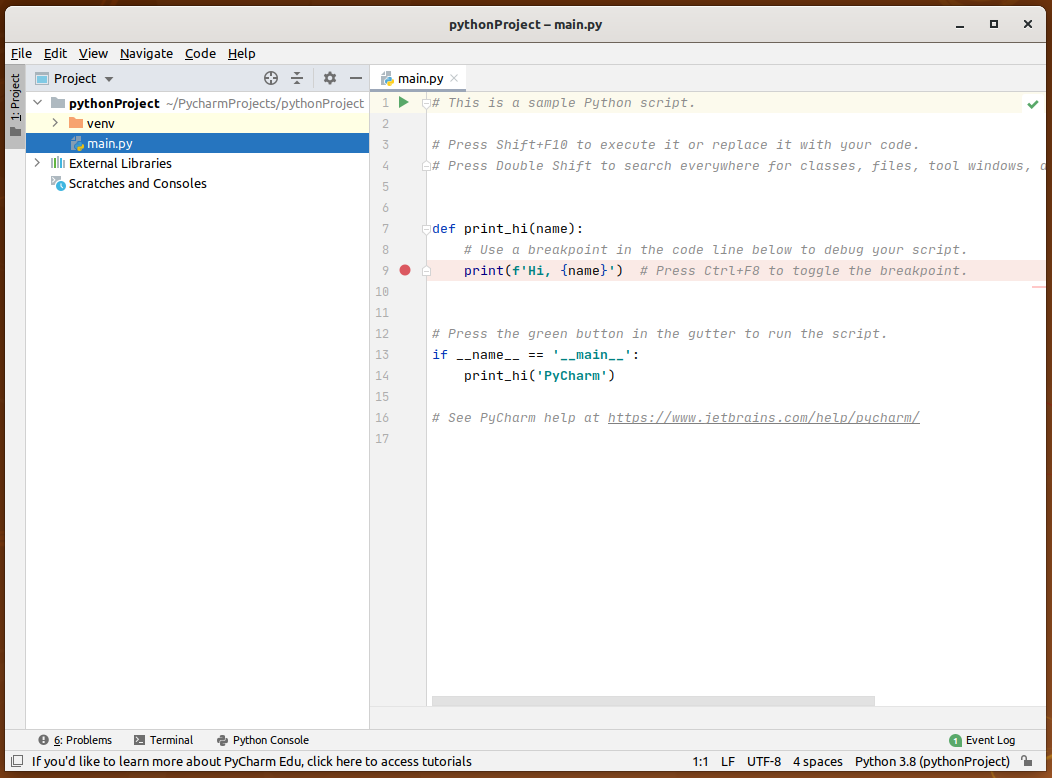
\includegraphics[height=0.8\textheight]{figs/pycharm.png}
    \caption{Gränssnittet för PyCharm.}
  \end{figure}
\end{frame}


\section{Hello World!}

\begin{frame}[fragile]
  \begin{example}
    \begin{minted}{python}
# Skriver ut till skärmen
print("Hello, World!")
    \end{minted}
  \end{example}

  \pause

  \begin{example}
    \begin{minted}{python}
# Skriver ut "Hello" + namnet till skärmen
name = "World"
print(f"Hello {name}!")
    \end{minted}
  \end{example}
\end{frame}

\begin{frame}[fragile]
  \begin{example}
    \begin{minted}{python}
# Skriver ut "Hello" + namnet till skärmen
name = "World"
print(f"Hello {name}!")
    \end{minted}
  \end{example}

  \pause

  \begin{example}[Funktioner]
    \begin{minted}{python}
def print_hello(name):
  """Skriver ut till skärmen"""
  print(f"Hello, {name}!")

print_hello("World")
    \end{minted}
  \end{example}
\end{frame}

